\chapter{Inheritance and polymorphism}

\section{PIE properties}

Object Oriented Programming (OOP) is a programming paradigm that uses objects to design 
applications and computer programs. It is based on several principles, the most important 
of which are the PIE properties:

\begin{itemize}
    \item \textbf{Polymorphism}: The ability of an object to take on many forms. The most 
    common use of polymorphism in OOP occurs when a parent class reference is used to refer 
    to a child class object.
    \item \textbf{Inheritance}: The mechanism by which one class acquires the properties and 
    behavior of another class. It supports the concept of hierarchical classification.
    \item \textbf{Encapsulation}: The mechanism that binds together the code and the data it 
    manipulates, and keeps both safe from outside interference and misuse.
\end{itemize}

\section{Inheritance}

Inheritance is a mechanism in which one class acquires the properties and behavior of 
another class. It supports the concept of hierarchical classification. Inheritance is 
a powerful feature of OOP that allows the creation of a new class that is based on an
existing class. The new class inherits the attributes and methods of the existing class,
and can also add new attributes and methods of its own.\\

When a class inherits from another class, there are three main benefits. You can:

\begin{itemize}
    \item Reuse code: The methods and attributes of the parent class are inherited by the 
    child class, so you don't have to write them again.
    \item Extend functionality: You can add new methods and attributes to the child class.
    \item Override functionality: You can override the methods of the parent class in the 
    child class.
\end{itemize}

In general, inheritance establishes an "is-a" relationship between the parent class and
the child class. For example, if you have a class called \texttt{Animal}, you could create
a child class called \texttt{Dog} that inherits from \texttt{Animal}. In this case, you could
say that a \texttt{Dog} is an \texttt{Animal}.\\

A derived class inherits every data member of the base class, as well as every ordinary
member function. However, the derived class does not inherit the constructors, 
destructor, or assignment operators of the base class, as well as the friend functions
of the base class, since these are class-specific.\\

In C++, inheritance is specified by the colon (\texttt{:}) followed by the access specifier
(public, protected, or private) and the name of the base class. The access specifier
determines the visibility of the base class members in the derived class. The default
access specifier is private. In this course we will only use public inheritance.\\

The syntax for inheritance is as follows:

\begin{lstlisting}[language=C++]
class Base {
    // Base class members
};

class Derived : public Base {
    // Derived class members
};
\end{lstlisting}

\subsection{Protected members and class access}

In C++, the protected access specifier is similar to the private access specifier, but
with one key difference: protected members are accessible in the derived class. This
means that a derived class can access the protected members of its base class, but an
object (instance) of the derived class cannot.\\

The protected access specifier is useful when you want to make the data members of the
base class accessible to the derived class, but not to the outside world. This allows
you to encapsulate the data members of the base class and provide controlled access to
them through the derived class.\\

The syntax for protected members is as follows:

\begin{lstlisting}[language=C++]
class Base {
protected:
    // Protected members
};

class Derived : public Base {
    // Derived class members
};
\end{lstlisting}

Note that protected members are only accessible for the derived class through the
derived class object. They are not accessible through the base class object.

\subsection{Creation and destruction of derived classes}

When a derived class object is created, the following steps occur:

\begin{itemize}
    \item Space is allocated for the full object, that is, enouch space to store the data
    members of both the base and derived classes.
    \item The base class constructor is called to initialize the base class data members.
    \item The derived class constructor is called to initialize the derived class data members.
    \item The derived class object is created and is now usable.
\end{itemize}

When a derived class object is destroyed, the following steps occur:

\begin{itemize}
    \item The derived class destructor is called to destroy the derived class data members.
    \item The base class destructor is called to destroy the base class data members.
    \item The space allocated for the object is deallocated.
\end{itemize}

\subsection{Class design principle}

In the absence of inheritance, we can think of a class as having two different kinds
of developers: the class designer and the class user. The first group is responsible
for designing the class, while the second group is responsible for using the class.\\

When inheritance is used, there is a third group of developers: the class extender. This
group is responsible for extending the class by adding new attributes and methods to it.
The class extender is also responsible for overriding the methods of the base class.\\

When implementing inheritance, it is important to be strictest as possible with the
access specifiers. The base class should have all its members private, except for the
methods that are meant to be overridden by the derived class. These methods should be
protected. The derived class should have all its members private, except for the methods
that are meant to be used by the class user. These methods should be public.

\section{Polymorphism}

Polymorphism is the ability of objects to respond in different ways to the same message or
function call. An object has "multiple identities", based on its class inheritance tree, meaning
it can be use in different ways depending on the context.\\

There are two types of polymorphism: compile-time polymorphism and run-time polymorphism.\\

\textbf{Compile-time polymorphism} is achieved through function overloading and function
redefinition. Function overloading allows you to define multiple functions with the same
name but different parameter lists. Function redefinition allows you to define a function
with the same name and parameter list in a derived class as in the base class, to change
the behavior of the function.\\

\textbf{Run-time polymorphism} is achieved through virtual functions and inheritance. Virtual
functions are functions that are declared in the base class and can be overridden by the
derived class. When a virtual function is called through a base class pointer or reference,
the function that is called is determined by the type of the object, not the type of the
pointer or reference.\\

\subsection{Virtual functions}

In \texttt{C++}, a base class distinguishes functions that are type dependant from those that
it expects its derived classes to inherit withou modification. The former are declared as
\texttt{virtual} functions. A virtual function is a member function that is declared in the
base class using the keyword \texttt{virtual}. A virtual function can be overridden by a
derived class to provide a different implementation.\\

A derived class may or may not override a virtual function. If it does not override the
virtual function, the base class version of the function is used. If it does override the
virtual function, the derived class version of the function is used.\\

An important thing to notice is that virtual member functions support dynamic binding. This
means that the function bounds to the object at runtime, not at compile time. Without 
virtual member functions, \texttt{C++} uses static binding, which means that the function
bounds to the object at compile time, and it is only considered function redefinition.\\

The syntax for virtual functions is as follows:\\

\begin{lstlisting}[language=C++]
class Base {
public:
    virtual void function() {
        // Base class implementation
    }
};

class Derived : public Base {
public:
    void function() override {
        // Derived class implementation
    }
};
\end{lstlisting}

Through dynamic binding, we can use the same code to process objects of the base class and
objects of the derived class. This is a powerful feature of \texttt{C++} that allows us to
write more flexible and maintainable code. It is also a key feature of polymorphism.\\

Note that polymorphic behavior is only possible when using pointers or references to objects.
When using objects directly, the function that is called is determined by the type of the
object, not the type of the pointer or reference. Look at the following example:\\

\begin{lstlisting}[language=C++]
#include <iostream>

class Base {
public:
    virtual void function() {
        std::cout << "Base class implementation" << std::endl;
    }
};

class Derived : public Base {
public:
    void function() override {
        std::cout << "Derived class implementation" << std::endl;
    }
};

void f(Base& b) {
    b.function();
}

int main() {
    Base b;
    Derived d;

    f(b);
    f(d);

    return 0;
}

// Output:
// Base class implementation
// Derived class implementation
\end{lstlisting}

To summarize, a base class specifies that a member function should be dynamically bound by
declaring it as virtual. A derived class specifies that it intends to override a virtual
function by using the \texttt{override} keyword. Any non-static member function, other than
a constructor, can be declared as virtual.\\

Note that, when a derived class overrides a virtual function, it may, but is not required to,
repeat the \texttt{virtual} keyword. This is a good practice, as it makes the code more readable, but 
once a function is declared as virtual in a base class, it remains virtual in all derived classes.\\

A derived-class function that overrides an inherited virtual function must have exactly the same 
parameter type(s) as the base-class function that it overrides. If the parameter types differ, the
functions are considered to be overloaded, not overridden.\\

With one exception, the return type of a virtual in the derived class must also match the return type
of the base-class function. The exception is that the return type of the derived-class function can be
a pointer or reference to a derived class type, even if the return type of the base-class function is
a pointer or reference to a base class type. I.e., if \texttt{D} is derived from \texttt{B}, then a base 
class virtual can return \texttt{B*} and the version of the derived can return \texttt{D*}.\\

\subsection{Derived-to-base conversion}

In \texttt{C++}, a derived class object can be assigned to a base class pointer or reference.
This is known as derived-to-base conversion. Derived-to-base conversion is useful when you
want to treat a derived class object as a base class object.\\

When a derived class object is assigned to a base class pointer or reference, only the base
class part of the object is accessible. This means that you can only access the base class
members of the object, not the derived class members.\\

For example:\\

\begin{lstlisting}[language=C++]
#include <iostream>

class Base {
public:
    virtual void function() {
        std::cout << "Base class implementation" << std::endl;
    }
};

class Derived : public Base {
public:
    void function() override {
        std::cout << "Derived class implementation" << std::endl;
    }
};

int main() {
    Derived d;
    Base* b = &d;

    b->function();

    return 0;
}

// Output:
// Derived class implementation
\end{lstlisting}

The fact that we can bind a reference or pointer to a base class object to a derived class
has an important implication: we don't know the actual type of the object to which the pointer
or reference is bound. This is a key feature of polymorphism. Tha object can be of the base
class type or of any derived class type.\\

We will deepen about this topic later in this chapter.

\subsection{Static and dynamic types}

In \texttt{C++}, an object has two types: a static type and a dynamic type. The static type
of an expression is the type that is known at compile time, it is the the type with which
a variable is declared. The dynamic type of an expression is the type that is determined at
runtime, it is the type of the object to which a pointer or reference is bound.\\

When a base class pointer or reference is bound to a derived class object, the static type
of the pointer or reference is the base class type, and the dynamic type of the object is
the derived class type. This means that the compiler treats the object as if it were of the
base class type, but the object behaves as if it were of the derived class type.\\

It is important to notice that the dynamic type of an expression that is neither a pointer
nor a reference is always the static type.\\

In the previous example, the static type of the pointer \texttt{b} is \texttt{Base*}, and the
dynamic type of the object to which \texttt{b} is bound is \texttt{Derived}. This is why the
function that is called is the \texttt{Derived} class implementation.

\section{Abstract classes}

An abstract class is a class that cannot be instantiated, that is, you cannot create an object
of an abstract class. An abstract class is used as a base class for other classes, and it is
designed to be inherited by other classes. An abstract class is a class that contains one or
more pure virtual functions.

\subsection{Pure virtual functions}

A pure virtual function is a virtual function that is declared in the base class but has no
implementation. A pure virtual function is declared using the syntax \texttt{virtual void function() = 0;}.
A pure virtual function must be overridden by a derived class to provide an implementation.\\

For example:\\

\begin{lstlisting}[language=C++]
#include <iostream>

class Base {
public:
    virtual void function() = 0;
};

class Derived : public Base {
public:
    void function() override {
        std::cout << "Derived class implementation" << std::endl;
    }
};

int main() {
    Derived d;

    d.function();

    return 0;
}

// Output:
// Derived class implementation
\end{lstlisting}

In this example, the \texttt{Base} class is an abstract class because it contains a pure virtual
function. The \texttt{Derived} class is a concrete class because it provides an implementation
for the pure virtual function. The \texttt{Derived} class can be instantiated, but the \texttt{Base}
class cannot.

\subsection{Refactoring}

When refactoring a class, it is important to consider the following:

\begin{itemize}
    \item If a class is not meant to be instantiated, make it an abstract class by adding
    a pure virtual function.
    \item If a class is meant to be instantiated, make it a concrete class by providing
    an implementation for the pure virtual function.
    \item If a class is meant to be inherited by other classes, make it a base class by
    adding virtual functions.
    \item If a class is meant to be used by other classes, make it a utility class by
    adding static functions.
\end{itemize}

By following these guidelines, you can create a well-structured class hierarchy that is
easy to understand and maintain.

\section{Derived-to-base conversion}

As we said before, because a derived object contains subparts corresponding to its base class(es),
we can use an object of a derived type as if it were an object of its base type(s). In particular,
we can binde a base-class reference or pointer to the base-class part of a derived object.

\begin{figure}[H]
    \centering
    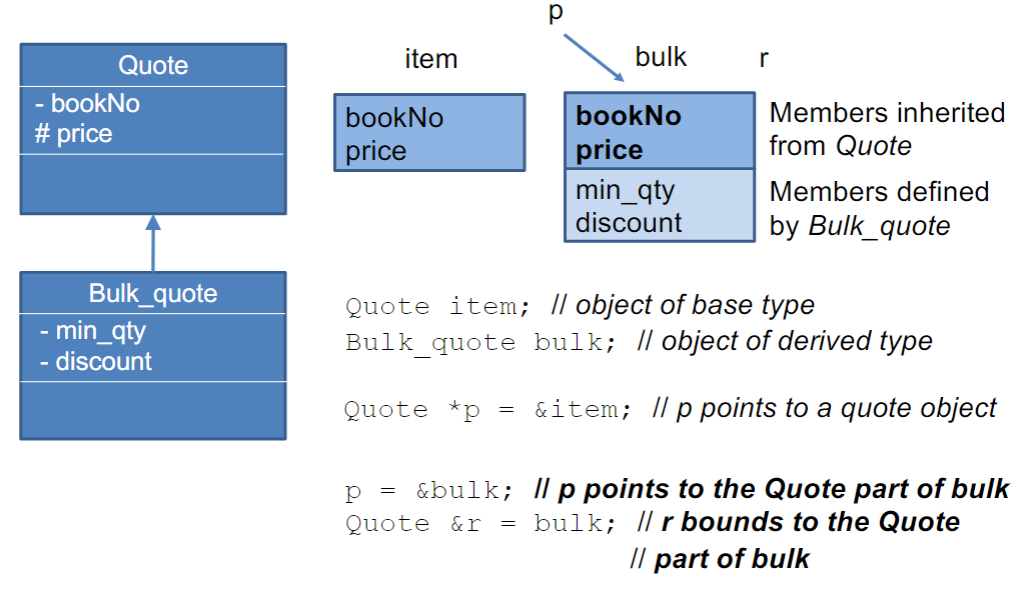
\includegraphics[width=12cm]{figures/derived-to-base_conv.png}
    \caption{Example of derived-to-base conversion}
    \label{fig:derived-to-base}
\end{figure}

Ordinarily, we can only bind a reference or a pointer to an object that has the same type as 
the corresponding reference or pointer. Classes related by inheritance are an important exception
of this rule.\\

The conversion from derived to base exists because every derived object contains a base-class 
part to which a pointer or reference of the base-class type can be bound. Note that there is
\textbf{no similar guarantee for base-class objects}. \\

A base-class object can exist either as an independent object or as a part of a derived object.
A base object that is not part of a derived object has only the members defined by the class;
it doesn't have the members defined by the derived class, i.e, \textbf{there is no automatic 
conversion} from the base class to the derived class.\\

\subsection{No conversion between objects}

Also note that the automatic derived-to-base conversion applies only for conversions to a reference
or pointer type. It is possible to convert an object of a derived class to its base-class type, but
such conversions may not behave as we might want.\\

When we initialize or assign an object of a class type, we are actually calling a function:
\begin{itemize}
    \item When we \textbf{initialize}, we're calling a \textbf{copy constructor}
    \item When we \textbf{assign}, we're calling an \textbf{assignment operator}
    \item These members normally have a parameter that is the reference to the const version of
    the class type.
\end{itemize}

Because these members take references, the derived-to-base conversion lets us pass a derived object
to a base-class copy operation.\\

\textbf{IMPORTANT!} These operations are \textbf{not virtual}. When we pass a derived object to a 
base-class constructor, the constructor that is run is defined in the base class. If we assign a 
derived object to a base object, the assignment operator that is run is defined in the base class.

\section{Containers and Inheritance}

When we use a container to store objects from an inheritance hierarchy, we generally must store
those objects indirectly. This is because the container must store objects of a single type, and
the objects in the hierarchy are of different types.\\

As an example, assume we want to define a vector to hold several books that a customer wants to buy.
We can't use a vector that holds \texttt{ScienceBook} objects, as we can't convert a \texttt{ScienceBook}
object to a \texttt{Book} object. We also can't use a vector that holds \texttt{Book} objects, because
if we add a \texttt{ScienceBook} object to the vector, we'll lose the \texttt{ScienceBook}-specific
information.\\

The solution is to use a vector of pointers to the base class. This way, we can store pointers to
objects of the derived classes in the vector, and we can access the objects through the base-class
interface. This is an example of dynamic binding, which is a key feature of polymorphism. Prefer
smart pointers to raw pointers.\\